% \documentclass[12pt,a4paper]{article}
\documentclass[12pt,a4paper]{article}
\usepackage[utf8]{inputenc}
\usepackage[T1]{fontenc}
\usepackage{lmodern} % load a font with all the characters
\usepackage[portuguese]{babel}
\usepackage{indentfirst}
\usepackage{listings}
\usepackage{amsmath}
\usepackage{mathtools}
\usepackage{tablefootnote}
\usepackage{graphicx}
\usepackage{csquotes}
\usepackage[section]{placeins}

\newcommand{\BigO}[1]{\ensuremath{\operatorname{O}\bigl(#1\bigr)}}

\title{Relatório EP2 - MAC0122 2015}
\author{
	Luca Serafini\\
	\texttt{No. USP 9373434}
	\and
	Lucas Santos\\
	\texttt{No. USP 9345064}
	\and
	Mardem Junior\\
	\texttt{No. USP 9065976}
}

\lstset{
  language=C,
  numbers=left,
  stepnumber=1,
  numbersep=5pt,
  showspaces=false,
  showstringspaces=false,
  showtabs=false,
  tabsize=2,
  captionpos=b,
  breaklines=true,
  breakatwhitespace=true,
  title=\lstname,
  inputencoding=utf8,
  extendedchars=true,
  literate=%
  {é}{{\'{e}}}1
  {è}{{\`{e}}}1
  {ê}{{\^{e}}}1
  {ë}{{\¨{e}}}1
  {É}{{\'{E}}}1
  {Ê}{{\^{E}}}1
  {û}{{\^{u}}}1
  {ù}{{\`{u}}}1
  {â}{{\^{a}}}1
  {à}{{\`{a}}}1
  {á}{{\'{a}}}1
  {ã}{{\~{a}}}1
  {Á}{{\'{A}}}1
  {Â}{{\^{A}}}1
  {Ã}{{\~{A}}}1
  {ç}{{\c{c}}}1
  {Ç}{{\c{C}}}1
  {õ}{{\~{o}}}1
  {ó}{{\'{o}}}1
  {ô}{{\^{o}}}1
  {Õ}{{\~{O}}}1
  {Ó}{{\'{O}}}1
  {Ô}{{\^{O}}}1
  {î}{{\^{i}}}1
  {Î}{{\^{I}}}1
  {í}{{\'{i}}}1
  {Í}{{\~{Í}}}1
}

\begin{document}
	\maketitle

	\section{Introdução}
	\indent O objetivo desse segundo exercício-programa (EP) consiste em desenhar uma árvore de decisão de diversos algoritmos de ordenação por comparação. Para isso, será utilizado a biblioteca gráfica desenvolvida no primeiro exercício-programa.\\
	\indent Os algoritmos que serão trabalhos nesse EP serão: selection sort, bubblesort, insertion sort, mergesort e heapsort. Adicionalmente, serão incluídas três implementações do quicksort: a primeira será da biblioteca padrão (stdlib), a segunda será uma implementação com aleatorização e a terceira sem aleatorização.\\
	\indent Nesse presente relatório explicaremos a solução desenvolvida, todas as complicações, otimizações e por fim, apresentaremos o resultado final, com desenhos e um manual de como usar o programa.


	\section{Algoritmos}
	\indent Abaixo descreveremos como cada algoritmo funciona, apresentaremos uma implementação em linguagem C e, por fim, seus respectivos tempos de execução (no pior, melhor e médio casos).\\
	\indent Na descrição dos algoritmos abaixo admitiremos que possuímos um vetor de inteiros V com N elementos. O objetivo será, portanto, ordenar o vetor V.\\
	\indent Assumiremos ainda que a implementação da função swap existe e seu funcionamento é realizar um intercâmbio dos valores de duas variáveis. Vamos utilizar as funções de comparação abaixo que serão exploradas no decorrer deste relatório:
	\begin{description}
	\item [greater(int a, int b):] retorna 1 se a é maior que b, 0 do contrário;
	\item [less(int a, int b):] retorna 1 se a é menor que b, 0 do contrário;
	\end{description}


	%%%%% %%%%% %%%%% %%%%% %%%%%
	% SELECTION SORT
	%%%%% %%%%% %%%%% %%%%% %%%%%
	\subsection{Selection sort}

	\subsubsection{Como funciona}
	\indent Esse algoritmo talvez seja o algoritmo mais ingênuo e fácil de ser entendido de todos que serão apresentados. Seu funcionamento é direto: seja i inicialmente igual a 0, itera-se o intervalo [i, N), buscando o menor elemento de índice u. Trocamos o elemento i com u e incrementamos i. Repetimos esse processo enquanto i for menor que N.

	\subsubsection{Implementação usual em C}
	\begin{minipage}{\linewidth}
	\begin{lstlisting}
	void selectionSort(int *v, int N) {
		int i, j, u;

		for (i = 0; i < N; i++) {
			u = i;
			for (j = i + 1; j < N; j++) {
				if (greater(v[u], v[j]))
					u = j;
			}

			swap(&v[u], &v[i]);
		}
	}
	\end{lstlisting}
	\end{minipage}

	\subsubsection{Tempo de execução}
	\indent No pior caso: \BigO{n^2}\\
	\indent No melhor caso: \BigO{n^2}\\
	\indent No caso médio: \BigO{n^2}



	%%%%% %%%%% %%%%% %%%%% %%%%%
	% BUBBLE SORT
	%%%%% %%%%% %%%%% %%%%% %%%%%
	\subsection{Bubble sort}

	\subsubsection{Como funciona}
	\indent O funcionamento desse algoritmo é também bem simples. Seja j = N-1, iteramos i no intervalo [0, j) comparando o i-ésimo elemento com o (i + 1)-ésimo elemento. Caso o i-ésimo elemento seja menor que seu sucessor, trocamos eles de posição e incrementamos i. Quando a iteração chegar ao fim, decrementamos j e repetimos o processo enquanto j for maior que 0. Uma implementação mais otimizada verifica se houve alguma troca. Caso não haja, significa que o vetor está ordenado e podemos parar. Essa otimização torna o tempo de execução do algoritmo em \BigO{n} no melhor caso.

	\subsubsection{Implementação usual em C}
	\begin{minipage}{\linewidth}
	\begin{lstlisting}
	void bubbleSort(int *v, int N) {
		int i, j, changed;

		for (j = N-1; j > 0; j -= 1) {
			changed = 0;

			for (i = 0; i < j; i++) {
				if (greater(v[i], v[i+1])) {
					swap(&v[i], &v[i+1]);
					changed = 1;
				}
			}

			if (changed == 0) break;
		}
	}
	\end{lstlisting}
	\end{minipage}

	\subsubsection{Tempo de execução}
	\indent No pior caso: \BigO{n^2}\\
	\indent No melhor caso: \BigO{n} quando otimizado\\
	\indent No caso médio: \BigO{n^2}



	%%%%% %%%%% %%%%% %%%%% %%%%%
	% INSERTION SORT
	%%%%% %%%%% %%%%% %%%%% %%%%%
	\subsection{Insertion sort}

	\subsubsection{Como funciona}
	\indent O mais eficiente dos algoritmos de ordenação com implementação mais simples (bubblesort e selection sort), seu funcionamento consiste em manter o início do vetor ordenado e a cada passo, insere um novo elemento na posição correta no intervalo já ordenado.

	\subsubsection{Implementação usual em C}
	\begin{minipage}{\linewidth}
	\begin{lstlisting}
	void insertionSort(int *v, int N) {
		int i, j, key;

		for (i = 1; i < N; i++) {
			key = v[i];
			j = i-1;
			while(j >= 0 && greater(v[j], key)) {
				v[j+1] = v[j];
				j -= 1;
			}
			v[j+1] = key;
		}
	}
	\end{lstlisting}
	\end{minipage}

	\subsubsection{Tempo de execução}
	\indent No pior caso: \BigO{n^2}\\
	\indent No melhor caso: \BigO{n}\\
	\indent No caso médio: \BigO{n^2}


	%%%%% %%%%% %%%%% %%%%% %%%%%
	% MERGESORT
	%%%%% %%%%% %%%%% %%%%% %%%%%
	\subsection{Mergesort}

	\subsubsection{Como funciona}
	\indent O algoritmo Mergesort utiliza a estratégia “dividir para conquistar”. Através de código recursivo, um vetor é dividido em várias seções menores, que, após serem ordenadas, são intercaladas, utilizando-se de um vetor auxiliar, de forma que o vetor todo estará em ordem crescente após a execução do algoritmo.\\
	\indent O algoritmo utiliza como base da recursão o fato de que um vetor com um elemento já está ordenado.

	\subsubsection{Implementação usual em C}
	\begin{lstlisting}
	void merge(int *v, int p, int q, int r) {
		int i, j, k, *aux;
		aux = malloc((r - p) * sizeof(int));
		i = p;
		j = q;
		k = 0;

		while (i < q && j < r) {
			if (greater(v[i], v[j])) aux[k++] = v[j++];
			else aux[k++] = v[i++];
		}

		while (i < q) aux[k++] = v[i++];
		while (j < r) aux[k++] = v[j++];
		
		for (i = p; i < r; i++) {
			v[i] = aux[i-p];
		}

		free(aux);
	}

	void mergesort(int *v, int p, int q) {
		if (p < q - 1) {
			int r = (p + q) / 2;
			mergesort(v, p, r);
			mergesort(v, r, q);
			merge(v, p, r, q);
		}
	}
	\end{lstlisting}

	\begin{minipage}{\linewidth}
	\subsubsection{Tempo de execução}
	\indent No pior caso: \BigO{n\log{}n}\\
	\indent No melhor caso: \BigO{n\log{}n}\\
	\indent No caso médio: \BigO{n\log{}n}
	\end{minipage}

	%%%%% %%%%% %%%%% %%%%% %%%%%
	% HEAPSORT
	%%%%% %%%%% %%%%% %%%%% %%%%%
	\subsection{Heapsort}

	\subsubsection{Como funciona}
	\indent O Heapsort utiliza a estrutura de dados chamada \textit{heap binário}, que fica escondida dentro dos vetores. Um (max) heap é um vetor v[1..m] tal que\\\\
	\centerline{v[f]  $\geq$  v[f/2]}\\\\
	para f = 2, ..., m. Vale ressaltar que f/2 deve ser entendido como $\lfloor f/2 \rfloor$. Nosso objetivo, nesse algoritmo, passa a ser transformar o vetor em um \textit{heap}.\\
	\indent Para isso, precisamos de uma função peneira que desça um elemento até sua posição correta. Somado a essa função, utilizamos uma segunda função, \textit{heapsort}, que desce, caso necessário, todos os elementos para as posições corretas.


	\subsubsection{Implementação usual em C}
	\begin{minipage}{\linewidth}
	\begin{lstlisting}
	void peneira(int *v, int p, int m) {
		int f = 2*p, x = v[p];
		
		while (f <= m) {
			if (f < m && less(v[f], v[f+1])) 
				f++;
			
			if (x >= v[f])
				break;
			
			v[p] = v[f];
			p = f;
			f = 2*p;
		}

		v[p] = x;
	}

	void heapsort(int *v, int n) {
	   int p, m;

		for (p = n/2; p >= 1; p--)
			peneira(v, p, n);

		for (m = n; m >= 2; m--) {
			swap(&v[1], &v[m]);
			peneira(v, 1, m-1);
		}
	}
	\end{lstlisting}
	\end{minipage}

	\subsubsection{Tempo de execução}
	\indent No pior caso: \BigO{n\log{}n}\\
	\indent No melhor caso: \BigO{n\log{}n}\\
	\indent No caso médio: \BigO{n\log{}n}



	%%%%% %%%%% %%%%% %%%%% %%%%%
	% QSORT
	%%%%% %%%%% %%%%% %%%%% %%%%%
	\subsection{Quicksort (biblioteca padrão)}
	\indent O funcionamento assemelha-se ao do quicksort sem aleatorização, descrito a seguir, mas sua implementação exata tal como seu tempo de execução não é especificado. Descreveremos a implementação da função de comparação que é utilizada no qsort da biblioteca padrão:

	\begin{minipage}{\linewidth}
	\begin{lstlisting}
	int qsort_compare_func(const void * a, const void * b) {
		int res = less(*(int *)a, *(int *)b);
		return res ? -1 : 1;
	}
	\end{lstlisting}
	\end{minipage}

	\indent Como estamos trabalhando com um vetor de elementos onde não temos repetição de elementos, é seguro retornar apenas se um elemento é maior ou menor que o outro, ignorando o caso de igualdade.



	%%%%% %%%%% %%%%% %%%%% %%%%%
	% QUICKSORT SEM ALEATORIZAÇÃO
	%%%%% %%%%% %%%%% %%%%% %%%%%
	\subsection{Quicksort sem aleatorização}

	\subsubsection{Como funciona}
	\indent O Quicksort utiliza a estratégia de “dividir para conquistar”. A formulação do algoritmo nas palavras do professor Paulo Feofiloff, do IME-USP:\\\\
	\indent \indent “rearranjar um vetor v[p..r] de modo que todos os elementos pequenos fiquem na parte esquerda do vetor e todos os elementos grandes fiquem na parte direita.”\\\\
	\indent Essa formulação é feita recursivamente tendo como base o vetor nulo, que já está ordenado.

	\subsubsection{Implementação usual em C}
	\begin{minipage}{\linewidth}
	\begin{lstlisting}
	int separar(int *v, int p, int r) {
		int x = v[r], 
			i = p - 1, 
			j = 0;

		for (j = p; j < r; j++) {
			if (less(v[j], x)) {
				i++;
				swap(&v[i], &v[j]);
			}
		}

		swap(&v[i+1], &v[r]);

		return i + 1;
	}

	void quicksort(int *v, int p, int r, int random) {
		if (p < r) {
			int q = random == 1 ? separar_random(v, p, r) : separar(v, p, r);
			quicksort(v, p, q - 1, random);
			quicksort(v, q + 1, r, random);
		}
	}
	\end{lstlisting}
	\end{minipage}

	\subsubsection{Tempo de execução}
	\indent No pior caso: \BigO{n^2}\\
	\indent No melhor caso: \BigO{n\log{}n}\\
	\indent No caso médio: \BigO{n\log{}n}


	%%%%% %%%%% %%%%% %%%%% %%%%%
	% QUICKSORT COM ALEATORIZAÇÃO
	%%%%% %%%%% %%%%% %%%%% %%%%%
	\subsection{Quicksort com aleatorização}

	\subsubsection{Como funciona}
	\indent Como o nome já diz, o Quicksort é um algoritmo de rápida ordenação, sendo considerado um dos mais eficientes. Porém, sua eficiência é da ordem de \BigO{n^2} no pior caso, ou seja, quando o vetor está praticamente ordenado e o pivô é o menor ou maior número. Isso faz com que tal algoritmo seja comparado aos algoritmos elementares nesses casos raros. Para consertar o problema, o pivô pode ser escolhido aleatoriamente, através da função rand da biblioteca \textit{“stdlib.h”}, fazendo com que sua eficiência seja da ordem de \BigO{n\log{}n} no pior caso.

	\subsubsection{Implementação usual em C}
	\begin{minipage}{\linewidth}
	\begin{lstlisting}
	int separar_random(int *v, int p, int r) {
		int random = rand() % (r - p) + p;
		swap(&v[r], &v[random]);
		return separar(v, p, r);
	}
	\end{lstlisting}
	\end{minipage}\\
	\indent A implementação do Quicksort descrita no item anterior já suporta a versão randômica.

	\subsubsection{Tempo de execução}
	\indent No pior caso: \BigO{n\log{}n}\\
	\indent No melhor caso: \BigO{n\log{}n}\\
	\indent No caso médio: \BigO{n\log{}n}







	\section{Solução}
	\indent Para construirmos a solução final, isto é, gerar o arquivo de imagem da árvore, precisamos quebrar o problema em problemas menores. O funcionamento do programa funciona em algumas etapas:

	\begin{itemize}
	\item \textbf{Implementação dos algoritmos de ordenação:} os algoritmos de ordenação devem ser escritos corretamente (a implementação, contudo, já foi descrita no capítulo anterior);
	\item \textbf{Permutar todas as combinações possíveis:} Dado um N de entrada, precisamos gerar todas as permutações de um vetor com N elementos distintos;
	\item \textbf{Analisar o comportamento do algoritmo (geração da árvore de decisão):} dado um algoritmo inserido na entrada do programa, para cada permutação, precisamos ver como o algoritmo se comporta (quais decisões ele faz). Com isso, conseguimos construir uma árvore binária com as decisões do algoritmo escolhido;
	\item \textbf{Calcular as posições dos nós e arestas:} dado a árvore binária, precisamos de um algoritmo que calcule a posição no plano cartesiano de cada nó a ser inserido no desenho;
	\item \textbf{Gerar o desenho:} conhecendo as posições, usamos a biblioteca desenvolvida no exercício-programa 1 para criar nosso desenho (Drawing);
	\item \textbf{Salvar o arquivo de imagem (PGM):} possuindo o desenho (Drawing), podemos salva-lo em um arquivo de imagem;
	\item \textbf{Fim};
	\end{itemize}



	\subsection{Implementação dos algoritmos de ordenação}
	\indent As implementações dos algoritmos já foram descritas no capítulo anterior.



	\subsection{Permutar todas as combinações possíveis}
	\indent Dado um valor N, queremos saber quais são todas as permutações possíveis de um vetor com N elementos distintos. Por simplificação, os elementos do vetor serão de 1 à N (1, 2, …, N).\\
	\indent A utilidade de conhecermos todas as permutações na construção do nosso exercício-programa se resume a conhecer quais decisões são feitas pelo algoritmo escolhido para todas as possíveis entradas. Conhecendo todas as decisões tomadas a partir de todas as permutações, somos capazes de determinar a árvore de decisões.\\
	\indent Abaixo, temos uma implementação recursiva para gerar as permutações:

	\begin{minipage}{\linewidth}
	\begin{lstlisting}
	void processEachPermutation(int n, int *v, int index) {
		if (n == index) {
			/* Aqui, o vetor v é uma permutação válida. Podemos trabalhar com ele. */

		} else for (int j = index; j < n; j++) {
			swap(&elements[index], &elements[j]);
			processEachPermutation(n, v, index + 1);
			swap(&elements[index], &elements[j]);

		}
	}
	\end{lstlisting}
	\end{minipage}

	\indent O tempo de execução desse algoritmo é \BigO{n!}. O fato do tempo de execução do algoritmo crescer com base no fatorial, torna essa etapa muito lenta. E não é muito difícil entendermos isso: para N = 8, temos que 8! =  40.320 e para N = 9, temos que 9! = 362.880. Ao passo que N aumentou em apenas uma unidade, N! aumentou em 322.560.\\
	\indent No capítulo de \textbf{Otimizações} discutiremos o tempo de execução desse método, tal como uma implementação iterativa e uma implementação onde pré-calculamos e armazenamos todas as permutações possíveis.



	\subsection{Analisar o comportamento do algoritmo (geração da árvore de decisão)}
	\indent Agora que possuímos os algoritmos implementados e as permutações disponíveis, precisamos analisar e armazenar como cada permutação se comporta no algoritmo.\\
	\indent No capítulo de implementação dos algoritmos, esboçamos duas funções customizadas de comparação: “greater” e “less”. A vantagem de usarmos operadores customizadas aparece aqui. Utilizando operadores customizados podemos ir construindo a árvore diretamente ao usar esses operadores.\\
	\indent Seja “nó” uma estrutura de duas variáveis: “esquerda” (do tipo “nó”) e “direita" (do tipo “nó”).\\
	\indent No início do programa definimos a raiz da árvore como um nó e no início do algoritmo de ordenação definimos o nó atual apontando para a raiz da árvore. A cada comparação entre dois valores, “a” e “b”, temos duas possibilidades:
	\begin{itemize}
		\item Ir para a esquerda, caso “a” seja menor que “b”. Nesse caso, definimos o nó atual como o nó à esquerda do nó atual (caso não esteja alocado na memória, alocamos-o);
		\item Ir para a direita, caso contrário. Nesse caso, definimos o nó atual como o nó à direita do nó atual (caso não esteja alocado na memória, alocamos-o);
	\end{itemize}
	\indent A implementação dos métodos comparativos customizados nos ajuda a fatorar o código que implementa a ideia acima. Isso acontece porque todos os algoritmos que estamos trabalhando são algoritmos de ordenação por comparação e, inevitavelmente, serão feitas comparações entre dois valores em algum momento da execução dos algoritmos.\\
	\indent A implementação dos comparadores é feita da seguinte forma:\\
	\begin{minipage}{\linewidth}
	\begin{lstlisting}
	Node **curNode; /* variável global usada para apontar o nó atual */

	int less(int a, int b) {
		if (a < b) {
			if (!((*curNode)->left))
				(*curNode)->left = createNode();
			
			*curNode = (*curNode)->left;
		} else {
			if (!((*curNode)->right))
				(*curNode)->right = createNode();
			
			*curNode = (*curNode)->right;
		}
		return a < b;
	}

	int greater(int a, int b) {
		if (a < b) {
			if (!((*curNode)->left))
				(*curNode)->left = createNode();

			*curNode = (*curNode)->left;
		} else {
			if (!((*curNode)->right))
				(*curNode)->right = createNode();
			
			*curNode = (*curNode)->right;
		}
		return a > b;
	}
	\end{lstlisting}
	\end{minipage}
	\indent Um ponto interessante é o fato da variável “curNode” (que representa o nó atual) ser do tipo “Node **”. O uso do ponteiro duplo acontece pelo fato de estarmos alterando o valor para qual ponteiro ele aponta.\\
	\indent Outro ponto interessante que vale ressaltar é que o tempo de execução dessa etapa é exatamente igual ao do algoritmo escolhido, uma vez que fizemos apenas uma pequena alteração para rastrear as decisões que ele faz.



	\subsection{Calcular as posições dos nós e arestas}
	\indent O objetivo dessa etapa é calcular as larguras de cada árvore.\\
	\indent Aqui poderíamos gerar a imagem de uma árvore perfeitamente simétrica, omitindo os nós que não aparecem na árvore de decisão. Contudo, isso não seria uma boa solução, uma vez que a largura da imagem ficaria bem maior. Deixar a largura maior do que o necessário não é interessante, pois ocupa mais espaço na memória e, principalmente, porque o tempo de execução do programa fica maior. Isso acontece porque os segmentos de retas (arestas) que ligam dois nós (vértices) possuiriam um comprimento maior e o tempo de execução para escreve-los na matriz aumentaria. Vale notar que a matriz também deverá ser maior.\\
	\indent Dado que cada nó pode ser visto como uma raiz e, dessa forma, formando uma árvore, uma abordagem interessante para resolver esse problema é uma função recursiva. Dessa forma, a largura de uma árvore é dada pela soma das larguras das árvores à esquerda e à direita. E caso o nó seja uma folha, isto é, não apresentar nós à esquerda e à direita, então temos que sua largura é a largura de um nó (definimos essa condição como base da nossa recursão). 
	\indent Temos que a implementação da função recursiva é dada por:\\
	\begin{minipage}{\linewidth}
	\begin{lstlisting}
	void calculateWidth(Node *node, double scale_x, double thickness) {
		if (!node->left && !node->right) {
			node->width = SPACE_PER_NODE_X(thickness, scale_x);

		} else {
			double width = SPACE_HORIZONTAL;

			if (node->left) {
				calculateWidth(node->left, scale_x, thickness);
				width += node->left->width;
			}

			if (node->right) {
				calculateWidth(node->right, scale_x, thickness);
				width += node->right->width;
			}

			node->width = width;
		}
	}
	\end{lstlisting}
	\end{minipage}
	\indent Observação: foi adicionado a estrutura “Node” (nó) o atributo “width” do tipo \textit{double} para que fosse possível armazenarmos a sua largura.



	\subsection{Gerar o desenho}
	\indent Calculado o quanto espaço cada nó ocupa, agora precisamos definir as coordenadas cartesianas. O desafio aqui é saber quanto espaço foi ocupado pelos nós à esquerda para então ocuparmos o próximo espaço vazio.\\
	\indent Novamente, usaremos a mesma abordagem recursiva. A base da recursão é quando o nó não existe e portanto não precisamos inseri-lo.\\
	\begin{minipage}{\linewidth}
	\begin{lstlisting}
	void insertNode(Drawing d, Node *node, double offsetY, double offsetX, double scale_y, double thickness) {
		if (!node) return;

		add_circle(d, offsetX + node->width / 2.0, offsetY, RADIUS(thickness), thickness, 1);
		node->x = offsetX + node->width / 2.0;
		node->y = offsetY;

		if (node->left) {
			insertNode(d, node->left, offsetY + SPACE_PER_NODE_Y(scale_y), offsetX, scale_y, thickness);
			add_line_segment(d, node->x, node->y, node->left->x, node->left->y, thickness);
		}

		if (node->right) {
			insertNode(d, node->right, offsetY + SPACE_PER_NODE_Y(scale_y), offsetX + nodeWidth(node->left), scale_y, thickness);
			add_line_segment(d, node->x, node->y, node->right->x, node->right->y, thickness);
		}
	}
	\end{lstlisting}
	\end{minipage}	
	\indent O funcionamento desse algoritmo é bem simples: sabendo a largura das árvores filhas, tanto a da esquerda quanto a da direita, é possível inseri-las (recursivamente) passando como argumento da função recursiva o \textit{offset} horizontal e vertical. Sabendo os \textit{offsets}, sabemos a posição a ser desenhada.



	\subsection{Salvar o arquivo de imagem (PGM)}
	\indent Com o desenho (drawing) gerado possuindo todos os círculos (que representam os nós) e segmentos de retas (que representam as arestas), podemos simplesmente chamar a função “save\_pgm”, que foi desenvolvida no exercício-programa 1, passando como argumento o desenho gerado.



	\subsection{Fim}
	\indent O programa, nesse ponto, funciona corretamente. Agora no próximo capítulo vamos discutir otimizações no programa a fim de executá-lo em um tempo menor.




	\section{Otimização}

	\subsection{Permutar todas as combinações possíveis}
	\indent No capítulo anterior, especificamente na etapa 2, definimos um algoritmo recursivo para gerar todas as permutações de um vetor de N elementos. Na linguagem C, sabe-se que na maioria dos casos as funções recursivas são mais lentas que as funções iterativas.\\
	\indent Uma possível otimização no código poderia ser feito, trocando o algoritmo recursivo de permutação por um iterativo. Pesquisando sobre algoritmos iterativos que computam todas as permutações de um dado vetor, encontramos um algoritmo chamado “Counting QuickPerm”\footnote{QuickPerm http://www.quickperm.org} que possui a seguinte implementação:\\
	\begin{minipage}{\linewidth}
	\begin{lstlisting}
	void processEachPermutation(int n, int *v, int *p) {
	   int i, j, tmp; 

	   i = 1;   
	   while(i < n) {
	      if (p[i] < i) {
	         j = i % 2 * p[i];   
	         swap(&v[j], &v[i]);
	         p[i]++;             
	         i = 1;              
	      } else {               
	         p[i] = 0;           
	         i++;                
	      } 
	   } 
	}
	\end{lstlisting}
	\end{minipage}
	\indent Uma terceira possível implementação surge do fato do valor de N estar restrito dentre 2 e 9. Essa informação nos permite pré-calcular e memorizar todas as permutações, colocando-as direto na memória. O trade-off nesse caso seria o custo que teríamos de armazenar todas as permutações na memória. A quantidade de número inteiros que teríamos que armazenar podem ser calculados como o somatório de todas as possibilidades possíveis para todos os possíveis valores de N:
	\begin{align*}
		\sum_{n=2}^{9} n! = 409.112
	\end{align*}
	\indent Considerando que cada inteiro ocupe 4 bytes, concluímos que os 409.112 inteiros ocupariam 1.636.448 bytes, equivalente a 1.63mb. Essa quantidade de memória consumida não se tornaria um problema no caso desse exercício-problema. Essa alternativa torna-se, portanto, uma alternativa viável que avaliaremos a seguir.\\
	\indent Desenvolvemos três programas separados, um com o algoritmo recursivo, outro com o algoritmo iterativo e um terceiro usando memorização afim de comparar o tempo de execução, na prática, dos mesmos. Usando o comando “time” do terminal de um único computador, cronometramos o tempo de execução dos três programas cuja finalidade é iterar todas as combinações possíveis. O resultado pode ser visto abaixo:\\
	\begin{table}[h!]
	\centering
	\begin{tabular}{lccc}
	                & \textbf{Algoritmo Recursivo} & \textbf{Algoritmo Iterativo} & \textbf{Memorização\tablefootnote{O tempo calculado é somente de executar um loop N! vezes e desconsideramos o tempo gasto para pré-calcular os valores.}} \\
	\textbf{N = 8}  & 0m0.005s                     & 0m0.004s                     & 0m0.002s              \\
	\textbf{N = 9}  & 0m0.013s                     & 0m0.009s                     & 0m0.004s              \\
	\textbf{N = 10} & 0m0.122s                     & 0m0.039s                     & 0m0.011s              \\
	\textbf{N = 11} & 0m1.128s                     & 0m0.364s                     & 0m0.088s              \\
	\textbf{N = 12} & 0m13.586s                    & 0m4.684s                     & 0m1.017s             
	\end{tabular}
	\end{table}\\
	\indent Claramente o algoritmo recursivo é o menos eficiente, seguido do iterativo e sendo o método de pré-calcular, dentre as opções apresentadas, o melhor método. Entretanto, optamos utilizar o método iterativo por ser suficientemente rápido para o pior caso (quando N for igual a 9).



	\subsection{Imprimindo a árvore}
	\indent Conforme foi detalhado no capítulo anterior, especificamente na etapa 4, estudamos a implementação de dois algoritmos para gerar as posições dos nós e das arestas.\\
	\indent O primeiro algoritmo possui uma solução mais simplificada e um tanto quanto ingênua. Sua execução consiste em calcular a altura H máxima da árvore. Sabendo a altura máxima da árvore, sabemos que a base dela possuí no máximo $2^{H-1}$ nós. Com isso podemos determinar a largura da base. Esse algoritmo gera uma árvore de largura simétrica e isso é inconveniente uma vez que na base da árvore tem menos nós que $2^{H-1}$ em alguns casos, ocupando, dessa forma, mais espaço horizontalmente do que deveria.\\
	\indent O segundo algoritmo, implementado no capítulo anterior, calcula as larguras recursivamente e dessa forma sabemos precisamente o espaço que estamos usando, evitando desperdícios de espaço que poderiam levar a um tempo maior de execução, uma vez que a imagem a ser gerada seria maior.



	\subsection{Otimizando os algoritmos de ordenação}
	\indent Alguns algoritmos, como o bubble sort, possuem implementações mais eficientes que consomem um tempo menor em alguns casos (no caso do bubble sort, a implementação mais eficiente torna o tempo de execução no melhor caso em \BigO{n}). Nesse exercício-programa, contudo, evitamos buscar qualquer tipo de otimização nos algoritmos de ordenação, se limitando às implementações passadas em aula pelo professor. Com isso, garantimos ainda que a árvore de decisão será completa e correta.



	\subsection{Otimizando a biblioteca \textit{graphics} do EP 1}
	\indent Certamente uma boa implementação da função save\_pgm pode melhorar, e muito, o tempo de execução do programa no geral. Para o exercício-programa 1, usamos uma abordagem que satisfazia as seguintes etapas:
	\begin{itemize}
	\item Iterava a lista de círculos e segmentos de reta;
		\begin{itemize}
			\item Para cada elemento da lista, definia-se a submatriz retangular para a qual o elemento contribuí na coloração dos pixels;
			\item Itera-se a submatriz calculando a cor em relação ao elemento atual;
		\end{itemize}
	\item No final da iteração a matriz já possui as cores definidas;
	\item Imprimir a matriz no arquivo PGM e fim;
	\end{itemize}

	\indent Esse algoritmo certamente já é bem eficiente uma vez que ele evita percorrer a matriz inteira sempre que possível. Mas ainda assim a submatriz que é percorrida possui muitos índices que não interferem na imagem, isto é, índices onde a cor permanece inalterada.\\
	\indent Antes, para calcular um segmento, iteravamos a submatriz que continha o segmento. Contudo, descobrimos que a maneira mais otimizada possível seria percorrer somente os índices que fazem parte diretamente do elemento e que podem alterar a cor da imagem. Para calcular os índices relevantes, foi utilizado noções de geometria e trigonometria simples.\\
	\indent Abaixo temos ilustrações que mostram como era feito antes e depois.

	\begin{figure}[h!]
		\centering
		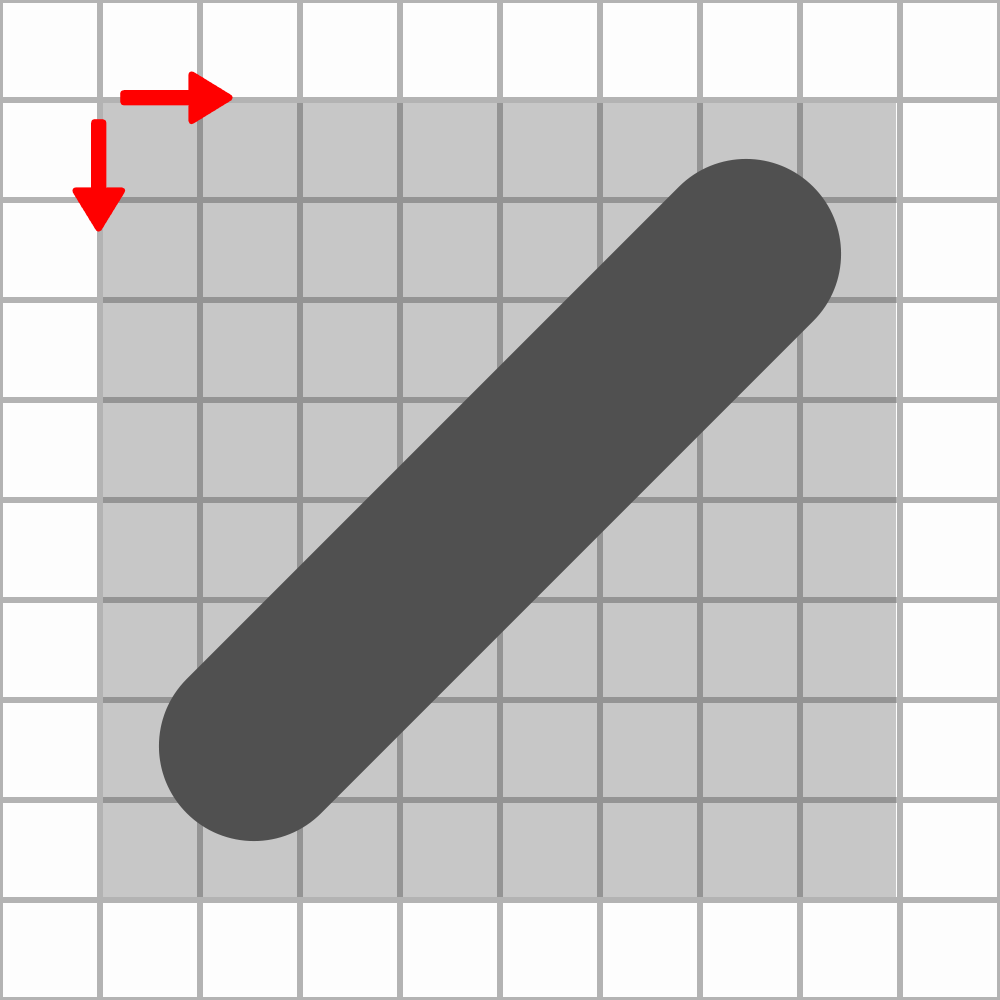
\includegraphics[height=6cm,keepaspectratio]{seg_antes.png}
		\caption{Antes}
	\end{figure}

	\begin{figure}[h!]
		\centering
		
\includegraphics[height=6cm,keepaspectratio]{seg_depois.png}
		\caption{Depois}
	\end{figure}


	\section{Desenhos}
	\indent Abaixo temos as imagens geradas pelo exercício-programa desenvolvido, para valores de N = 5 com as seguintes entradas:\\
	\begin{description}
	\item [Escala X] 1.0;
	\item [Escala Y] 1.0;
	\item [Grossura] 3.0;
	\item [Pixels por unidade] 10;
	\item [Tamanho da amostra] 3;
	\item [Tipo de amostra] grid;
	\end{description}

	\begin{figure}[h!]
		\vspace*{0.3in}
		\centering
		
\includegraphics[width=\textwidth]{insertion_sort.png}
		\caption{Insertion sort}
	\end{figure}

	\begin{figure}[h!]
		\vspace*{0.3in}
		\centering
		
\includegraphics[width=\textwidth]{bubble_sort.png}
		\caption{Bubble sort (com otimização)}
	\end{figure}

	\begin{figure}[h!]
		\vspace*{0.3in}
		\centering
		
\includegraphics[width=\textwidth]{selection_sort.png}
		\caption{Selection sort}
	\end{figure}

	\begin{figure}[h!]
		\vspace*{0.3in}
		\centering
		
\includegraphics[width=\textwidth]{qsort.png}
		\caption{Qsort (biblioteca padrão)}
	\end{figure}

	\begin{figure}[h!]
		\vspace*{0.3in}
		\centering
		
\includegraphics[width=\textwidth]{mergesort.png}
		\caption{Mergesort}
	\end{figure}

	\begin{figure}[h!]
		\vspace*{0.3in}
		\centering
		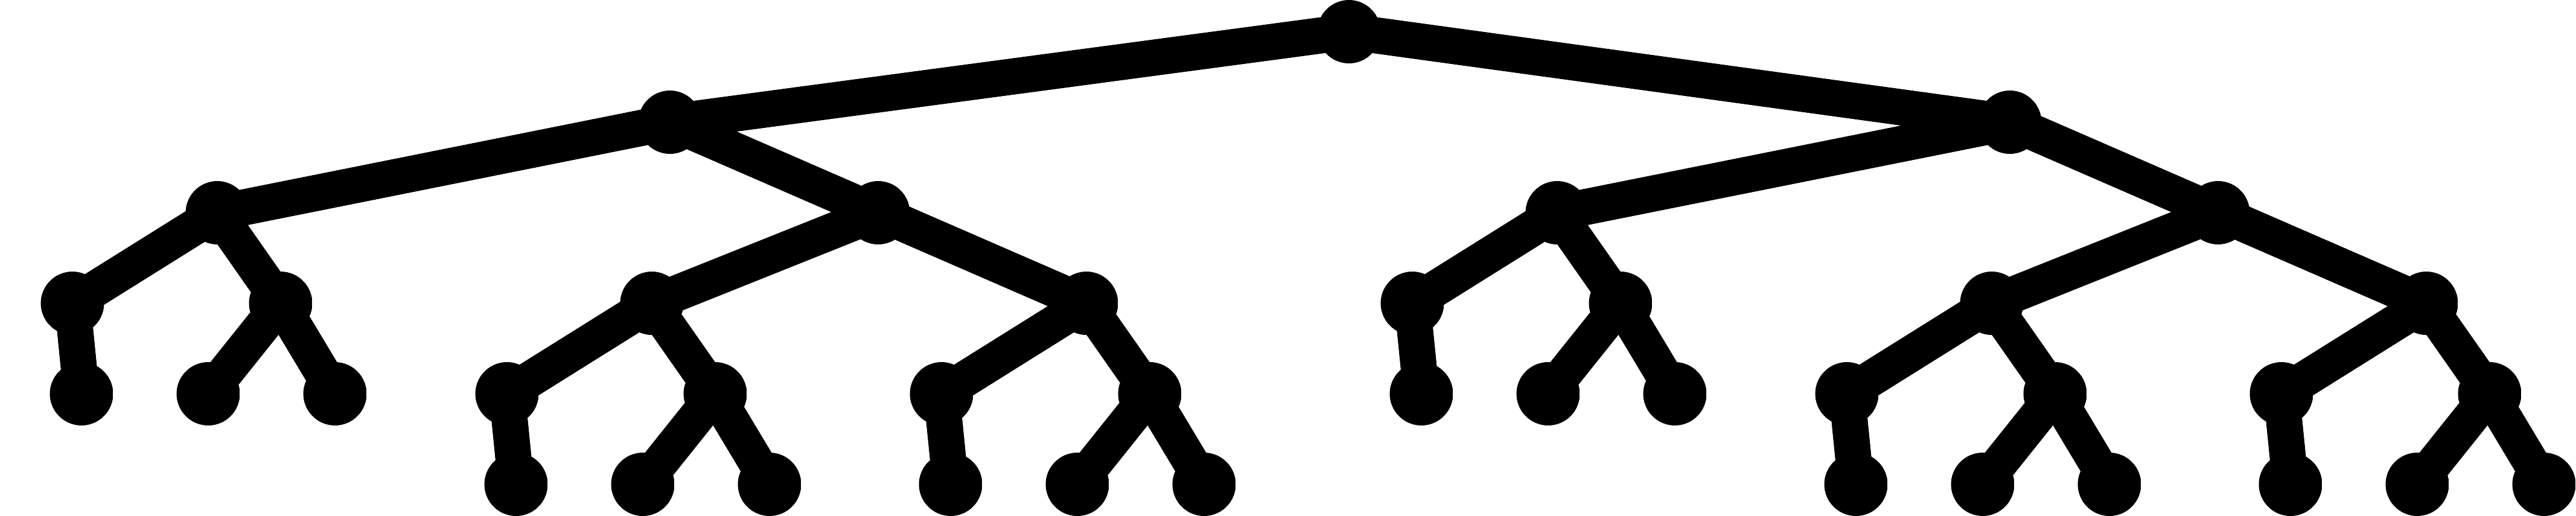
\includegraphics[width=\textwidth]{heapsort.png}
		\caption{Heapsort}
	\end{figure}

	\begin{figure}[h!]
		\vspace*{0.3in}
		\centering
		
\includegraphics[width=\textwidth]{quicksort.png}
		\caption{Quicksort sem aleatorização}
	\end{figure}

	\begin{figure}[h!]
		\vspace*{0.3in}
		\centering
		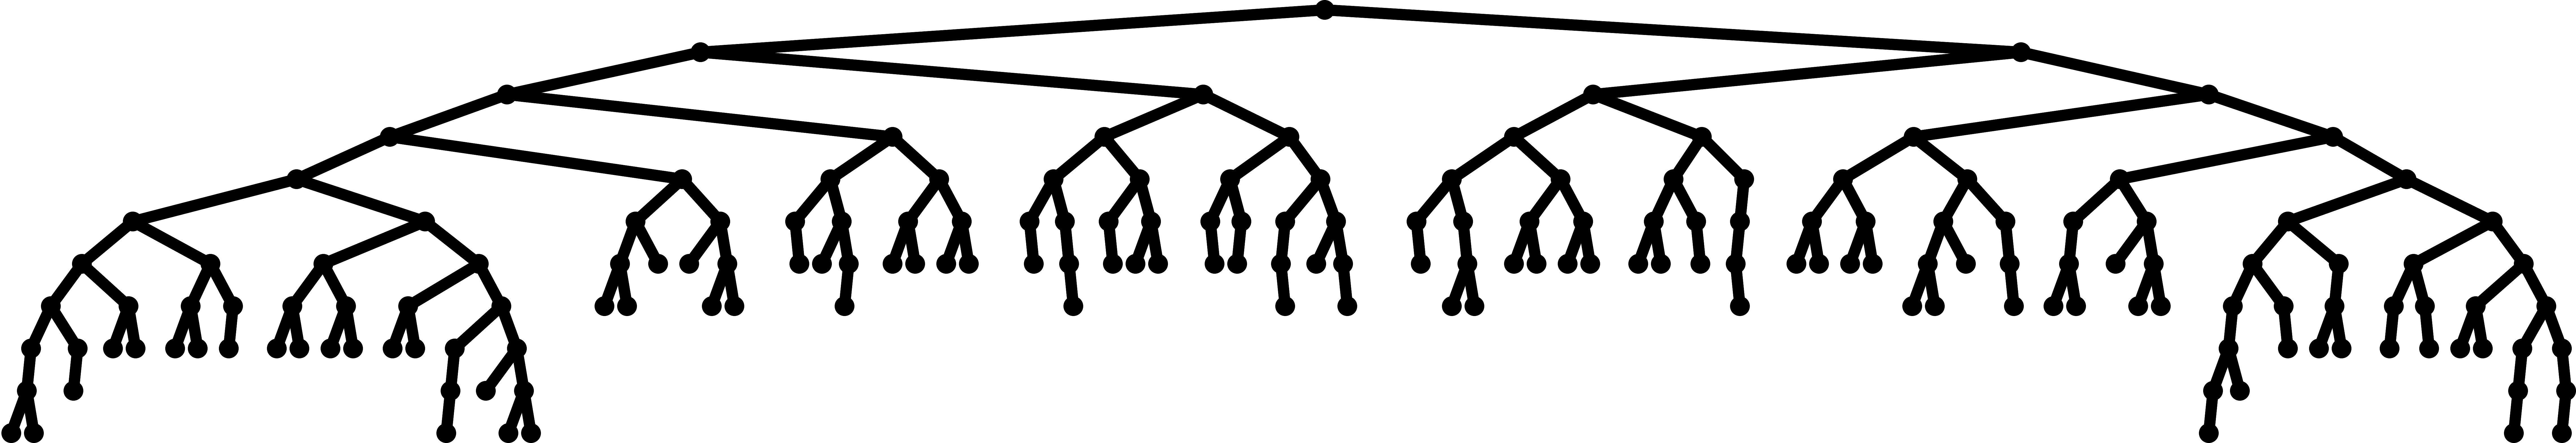
\includegraphics[width=\textwidth]{quicksort_random.png}
		\caption{Quicksort com aleatorização}
	\end{figure}




	\section{Manual de uso}

	\subsection{Estrutura dos arquivos}
	\indent A estrutura dos arquivos é bem simples. Segue a descrição do que cada arquivo é encarregado de fazer:
	\begin{enumerate}
	\item \textbf{builder} (.c, .h): calcular a largura de uma árvore, as posições de cada nó e aresta e, por fim, integrar com a biblioteca \textit{graphics};
	\item \textbf{graphics} (.c, .h): biblioteca escrita no EP 1 e otimizada agora, serve para criar desenhos e salvá-los no formato \textit{.pgm};
	\item \textbf{main} (.c): recebe as entradas pela linha de comando e dá início ao programa;
	\item \textbf{tree} (.c, .h): responsável por obter uma árvore de um algoritmo;
	\end{enumerate}

	\subsection{Compilando}
	\indent O exercício-programa conta com um arquivo Makefile que torna todo o processo de compilação mais simples. Para compilar, basta digitar no terminal “\textit{make}”. Isso já será o suficiente para compilar todos os arquivos, gerando o executável.\\

	\subsection{Como usar}
	\indent Esse exercício-programa foi feito para funcionar somente pela linha de comando, exatamente como foi feito no exercício-programa anterior. O uso se dá da seguinte forma:\\

	\indent \textbf{tree} <algoritmo> <num\_elementos> <outfile> <scale\_x> <scale\_y> <grossura> <pix\_por\_unidade> <tamanho\_amostra> <tipo\_amostra>\\

	\begin{itemize}
	\item \textit{algoritmo:} qual algoritmo a árvore deve representar. Disponivel: qsort, selection\_sort, insertion\_sort, bubble\_sort, quicksort\_random, quicksort, mergesort, heapsort;
	\item \textit{num\_elementos:} (número inteiro) número de elementos para ser sorteado. Tenha cuidado: evite escolher números altos (o programa ainda funcionará, mas seu tempo de execução cresce rapidamente);
	\item \textit{outfile:} nome do arquivo de saída que a imagem deve ser escrita;
	\item \textit{scale\_x:} (número real) fator escalar na largura (eixo X);
	\item \textit{scale\_y:} (número real) fator escalar na vertical (eixo Y);
	\item \textit{grossura:} (número real) grossura das linhas e dos nós;
	\item \textit{pix\_por\_unidade:} (número inteiro) número de pixels por unidade;
	\item \textit{tamanho\_amostra:} (número inteiro) tamanho da amostra;
	\item \textit{tipo\_amostra:} (opcional) ou “grid”, para um gride uniforme, ou “random” para um grid rândomico. Grid por padrão;
	\end{itemize}
	\indent A saída do programa se limita à geração do arquivo com nome igual à entrada no programa pelo parâmetro “outfile”.



\end{document}